% Volatility Arbitrage — Beamer Presentation
% MS&E 244, Stanford University
\documentclass[11pt]{beamer}
\usetheme{Madrid}
\usecolortheme{default}

% ── Custom color palette (match project figures) ─────────────
\definecolor{color50}{HTML}{FCE9E9}
\definecolor{color100}{HTML}{F6C1C1}
\definecolor{color200}{HTML}{F09999}
\definecolor{color300}{HTML}{EA7171}
\definecolor{color400}{HTML}{E44949}
\definecolor{color500}{HTML}{DE2121}
\definecolor{color600}{HTML}{B61B1B}
\definecolor{color700}{HTML}{8C1515}
\definecolor{color800}{HTML}{660F0F}
\definecolor{color900}{HTML}{3E0909}
\definecolor{color950}{HTML}{160303}

% Headers: white text on dark background
\setbeamercolor{structure}{fg=color700}
\setbeamercolor{palette primary}{bg=color700,fg=white}
\setbeamercolor{palette secondary}{bg=color800,fg=white}
\setbeamercolor{palette tertiary}{bg=color900,fg=white}
\setbeamercolor{frametitle}{bg=color700,fg=white}
\setbeamercolor{block title}{bg=color200,fg=color900}
\setbeamercolor{block body}{bg=color50,fg=color900}
\setbeamercolor{title in head/foot}{fg=white}
\setbeamercolor{author in head/foot}{fg=white}
\setbeamercolor{date in head/foot}{fg=white}
\setbeamercolor{section in head/foot}{fg=white}

% Frametitle: dark bar with white text
\setbeamertemplate{frametitle}{
  \nointerlineskip
  \vspace{0.3em}
  \begin{beamercolorbox}[wd=\paperwidth,leftskip=0.5cm,rightskip=0.5cm plus 1fil]{frametitle}
    \vbox to 0.8cm{\vfil\insertframetitle\vfil}
  \end{beamercolorbox}
  \vspace{0.2em}
}

% Footer: smaller font and constrained width to prevent overflow
\setbeamertemplate{footline}{
  \leavevmode%
  \hbox{%
  \begin{beamercolorbox}[wd=0.28\paperwidth,ht=2.25ex,dp=1ex,left,leftskip=0.5cm]{author in head/foot}%
    \raggedright\tiny\insertshortauthor
  \end{beamercolorbox}%
  \begin{beamercolorbox}[wd=0.44\paperwidth,ht=2.25ex,dp=1ex,center]{title in head/foot}%
    \centering\tiny\parbox{0.42\paperwidth}{\centering\insertsectionhead}
  \end{beamercolorbox}%
  \begin{beamercolorbox}[wd=0.28\paperwidth,ht=2.25ex,dp=1ex,right,rightskip=0.5cm]{date in head/foot}%
    \raggedleft\tiny\insertshortdate\hspace*{0.5em}\insertframenumber/\inserttotalframenumber
  \end{beamercolorbox}}%
  \vskip0pt%
}

\usepackage{booktabs}
\usepackage{amsmath}
\usepackage{multicol}
\usepackage{adjustbox}
\usepackage{tikz}
\usetikzlibrary{shapes.geometric,arrows.meta,positioning}
\graphicspath{{figures/}{../output/figures/}}

\title{Volatility Arbitrage via the Variance Risk Premium}
\subtitle{Trading the IV--Forecast RV Spread on SPX Options}
\author[Group 4]{Group 4 \\ MS\&E 244: Statistical Arbitrage}
\institute[Stanford]{Stanford University}
\date[W2026]{Winter 2026}

\begin{document}

\begin{frame}
  \titlepage
\end{frame}

% ═══════════════════════════════════════════════════════════
\section{Introduction}
% ═══════════════════════════════════════════════════════════

\begin{frame}{Motivation \& Strategy}
  \begin{columns}[T]
    \begin{column}{0.48\textwidth}
      \textbf{Motivation}
      \begin{itemize}
        \item \textbf{VRP:} Implied variance $>$ realized variance.
        \item Compensates sellers for crash risk.
        \item \textbf{Question:} Is IV--forecast RV spread tradeable?
      \end{itemize}
      \vspace{0.5em}
      \textbf{Strategy}
      \begin{itemize}
        \item Delta-hedged ATM straddles on SPX.
        \item Enter when VRP z-score $> 1$ (short vol) or $< -1$ (long vol).
        \item Hold to expiry (1--5d for weeklies); 25\% stop per trade (early exit \& expiry); \$1M notional, 5\,bps cost.
      \end{itemize}
    \end{column}
    \begin{column}{0.48\textwidth}
      \begin{adjustbox}{max width=\linewidth,max height=0.52\textheight,keepaspectratio}
        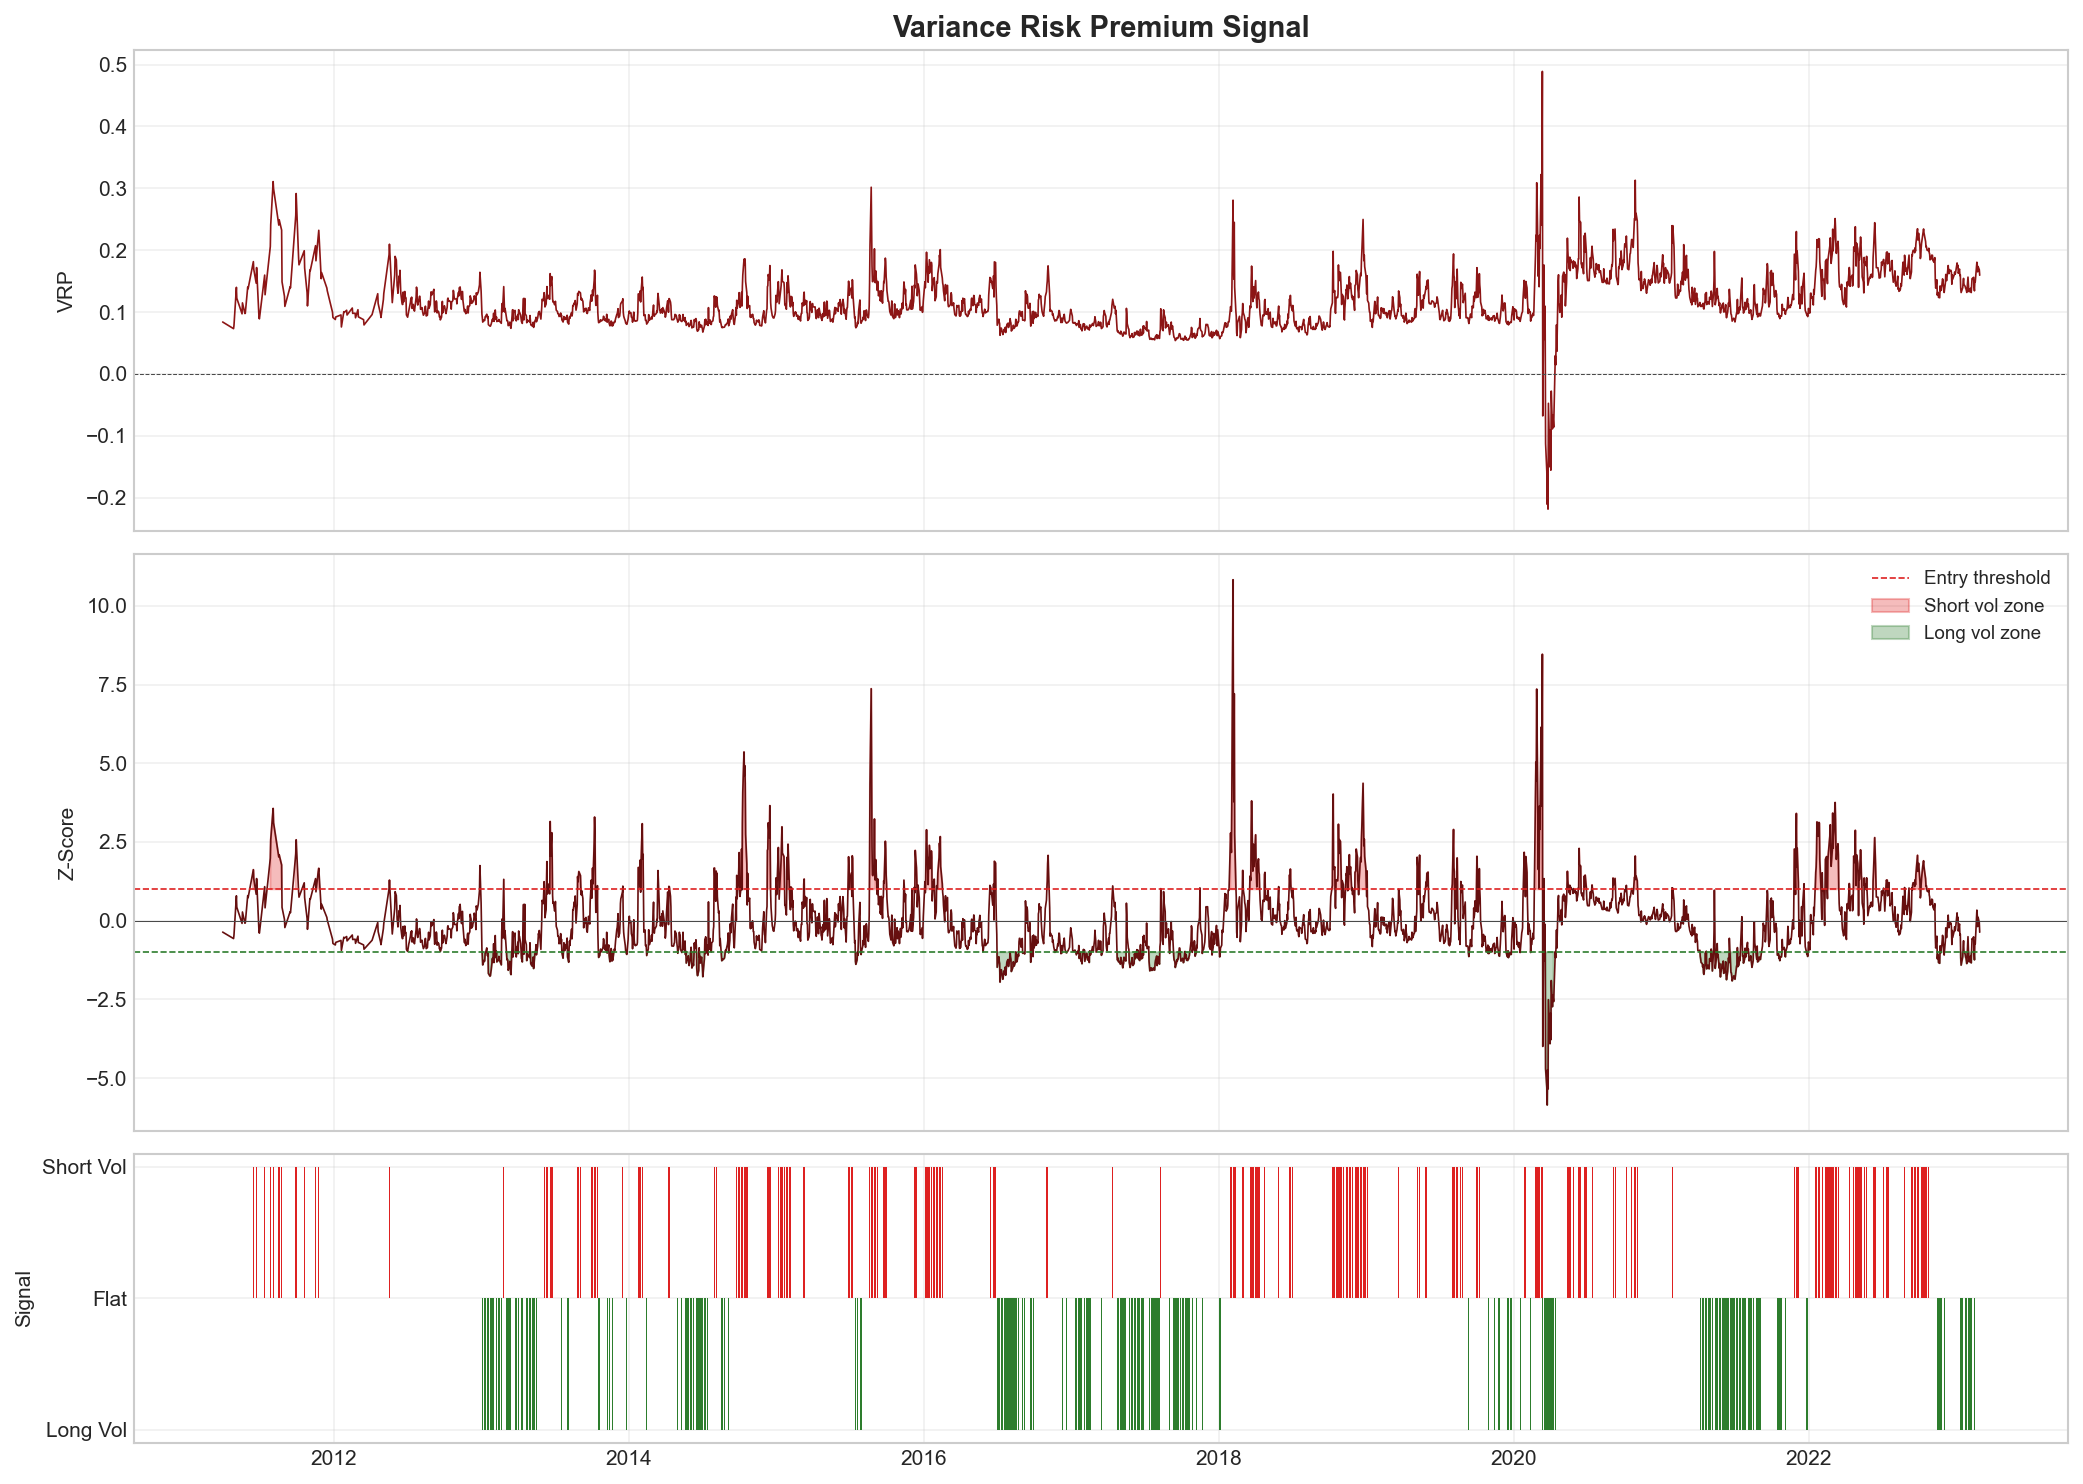
\includegraphics[width=\textwidth]{05_vrp_signal.png}
      \end{adjustbox}
      \vspace{-0.3em}
      \scriptsize VRP z-score and discrete signal.
    \end{column}
  \end{columns}
\end{frame}

% ═══════════════════════════════════════════════════════════
\section{Data \& Features}
% ═══════════════════════════════════════════════════════════

\begin{frame}{Data: SPX \& Options}
  \begin{columns}[T]
    \begin{column}{0.48\textwidth}
      \begin{adjustbox}{max width=\linewidth,max height=0.52\textheight,keepaspectratio}
        
\includegraphics[width=\textwidth]{01_spx_price_returns.png}
      \end{adjustbox}
      \vspace{-0.3em}
      \scriptsize SPX price and daily log returns.
    \end{column}
    \begin{column}{0.48\textwidth}
      \begin{adjustbox}{max width=\linewidth,max height=0.52\textheight,keepaspectratio}
        
\includegraphics[width=\textwidth]{02_options_summary.png}
      \end{adjustbox}
      \scriptsize Options: volume, IV, moneyness, DTE. OptionMetrics 2005--2023; filters on bid, spread, DTE 7--60, moneyness $\pm$20\%.
    \end{column}
  \end{columns}
\end{frame}

\begin{frame}{Strategies Compared (Methods \& Models)}
  \footnotesize
  \textbf{1. VRP (Variance Risk Premium)} — Level signal
  \begin{itemize}
    \item IV: ATM at expiry (1--5d); RV: HAR/GARCH/GJR composite forecast
    \item Signal: $z = (\text{IV} - \text{RV})/\sigma$; enter $|z| > 1$; short vol when IV rich
  \end{itemize}
  \vspace{0.2em}
  \textbf{2. Var Swap} — Model-free IV
  \begin{itemize}
    \item IV: MFIV at expiry (variance swap rate from full option surface)
    \item Same RV forecast and z-score rules; captures entire implied variance
  \end{itemize}
\end{frame}

\begin{frame}{IV vs RV \& RV Forecasts}
  \begin{columns}[T]
    \begin{column}{0.48\textwidth}
      \begin{adjustbox}{max width=\linewidth,max height=0.52\textheight,keepaspectratio}
        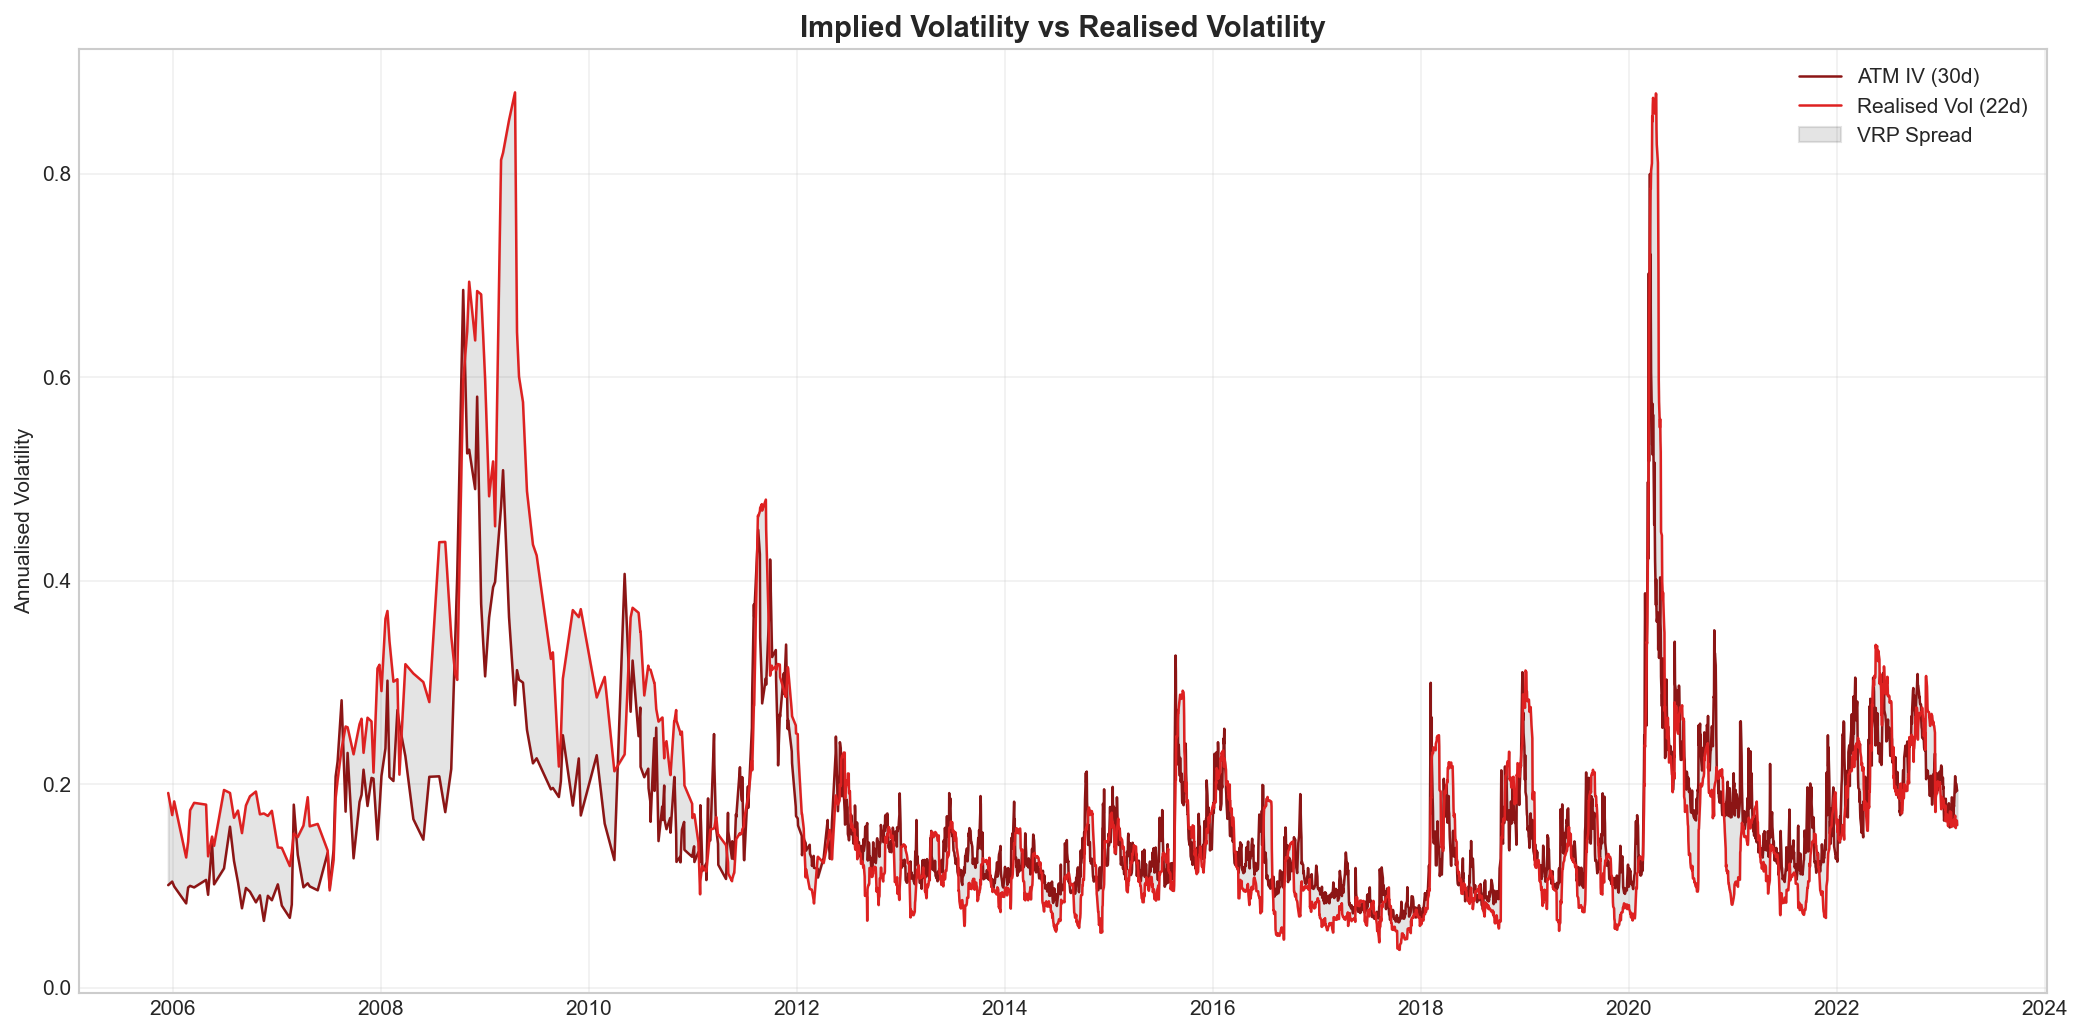
\includegraphics[width=\textwidth]{03_iv_vs_rv.png}
      \end{adjustbox}
      \vspace{-0.3em}
      \scriptsize ATM IV (at expiry) vs realized vol; spread = VRP raw input.
    \end{column}
    \begin{column}{0.48\textwidth}
      \begin{adjustbox}{max width=\linewidth,max height=0.52\textheight,keepaspectratio}
        
\includegraphics[width=\textwidth]{04_rv_forecasts.png}
      \end{adjustbox}
      \vspace{-0.3em}
      \scriptsize HAR-RV, GARCH, GJR vs actual forward RV; composite = equal-weight.
    \end{column}
  \end{columns}
\end{frame}

\begin{frame}{Signals: VRP \& Surface}
  \begin{columns}[T]
    \begin{column}{0.48\textwidth}
      \begin{adjustbox}{max width=\linewidth,max height=0.52\textheight,keepaspectratio}
        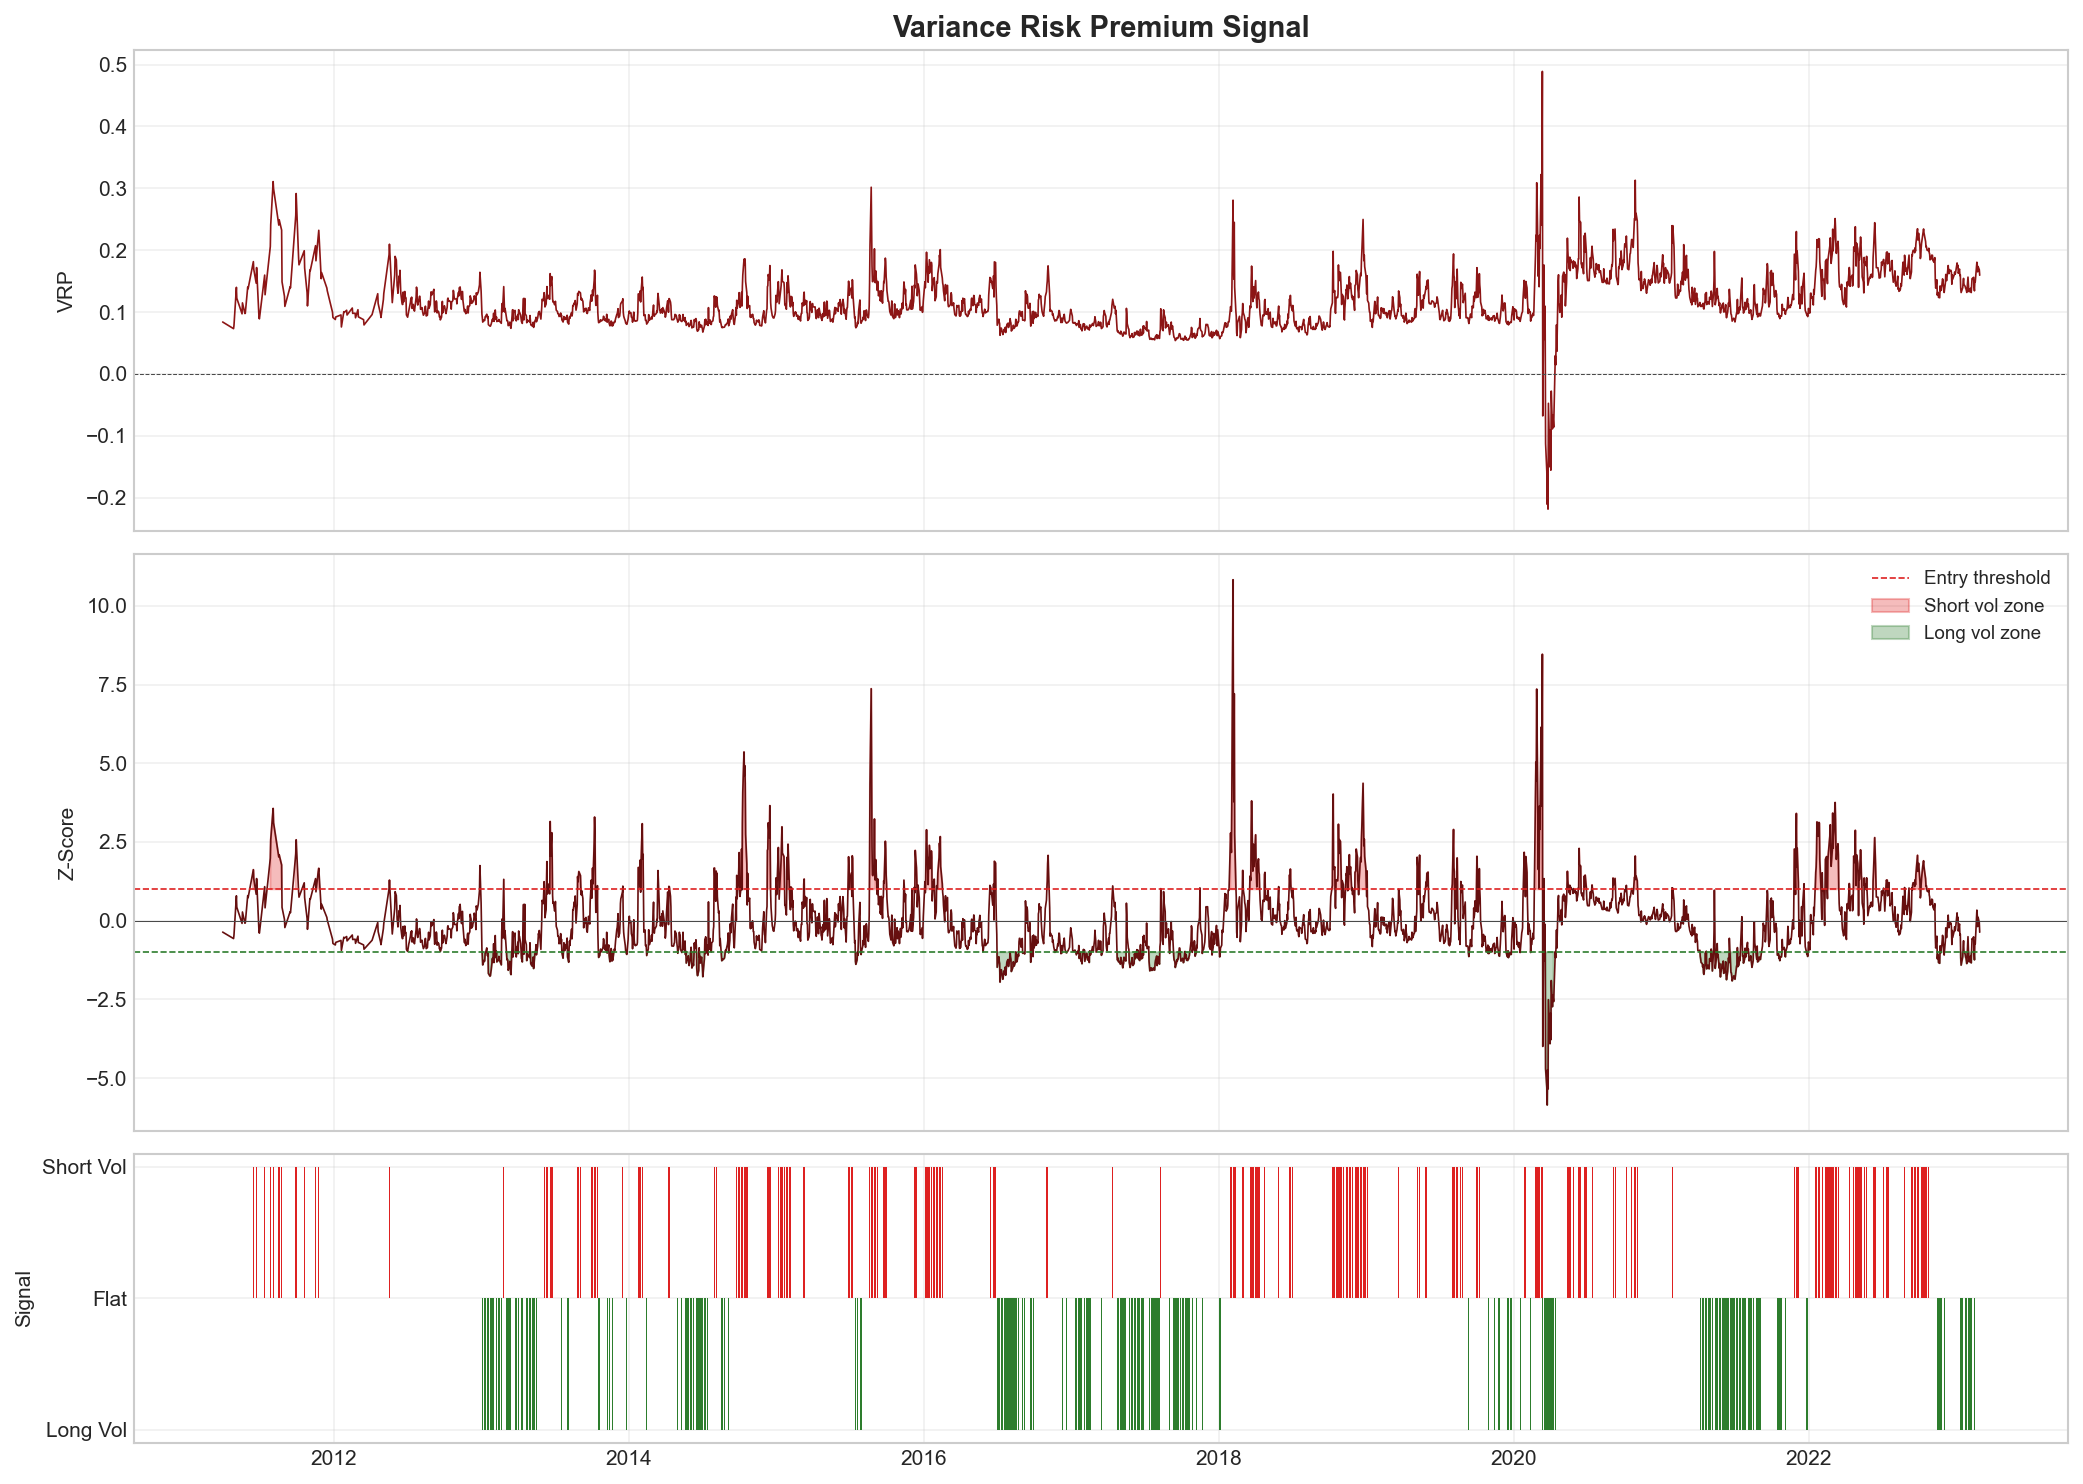
\includegraphics[width=\textwidth]{05_vrp_signal.png}
      \end{adjustbox}
      \vspace{-0.3em}
      \scriptsize VRP level, z-score, and $\pm 1$ entry bands.
    \end{column}
    \begin{column}{0.48\textwidth}
      \begin{adjustbox}{max width=\linewidth,max height=0.52\textheight,keepaspectratio}
        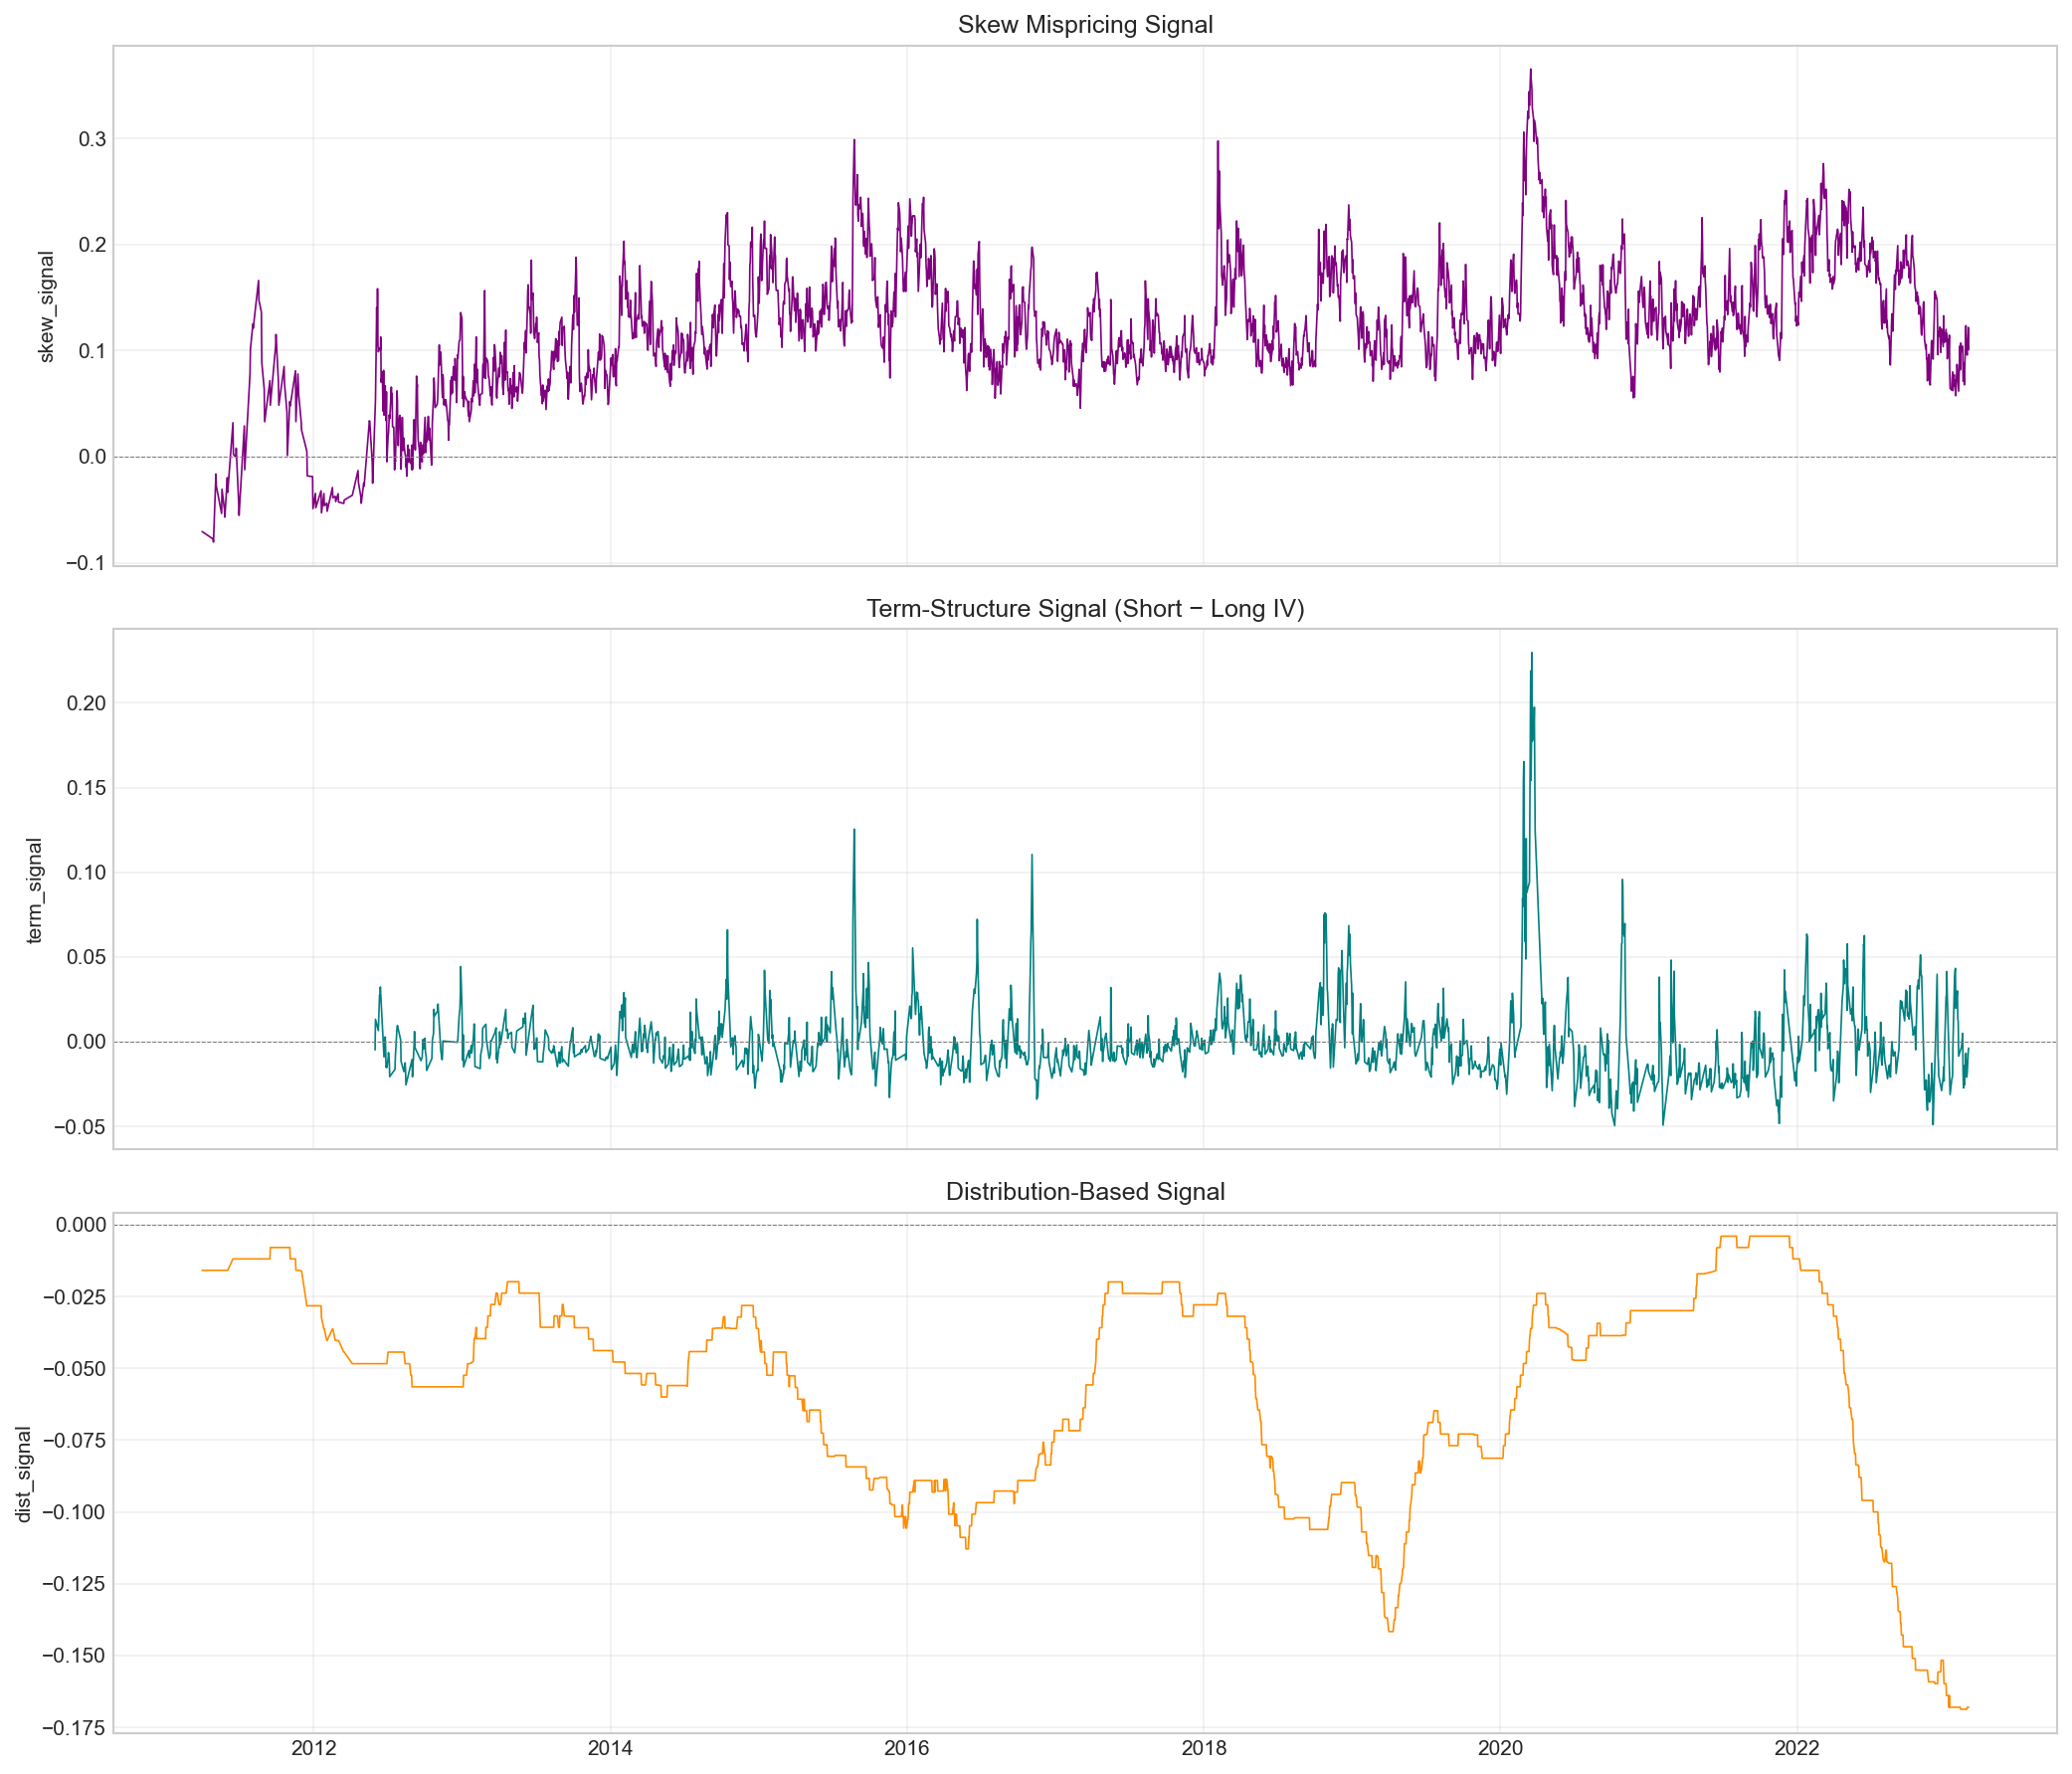
\includegraphics[width=\textwidth]{06_surface_signals.png}
      \end{adjustbox}
      \vspace{-0.3em}
      \scriptsize Skew and term-structure signals.
    \end{column}
  \end{columns}
\end{frame}

% ═══════════════════════════════════════════════════════════
\section{Logistic Regression (RV Forecast)}
% ═══════════════════════════════════════════════════════════

\begin{frame}{Logistic Regression: Methodology}
  \centering
  \begin{adjustbox}{max width=\textwidth,max height=0.52\textheight,keepaspectratio}
  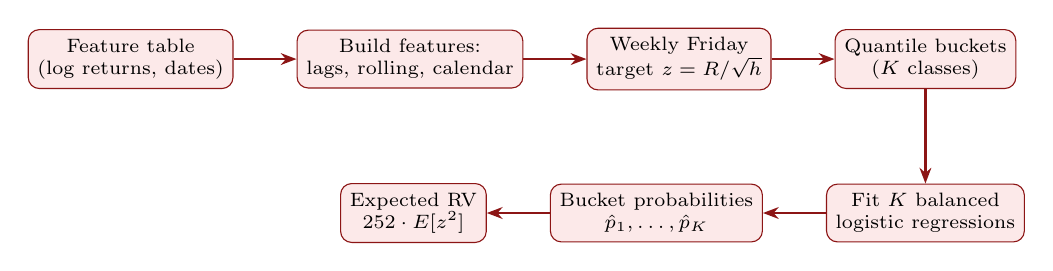
\begin{tikzpicture}[
    node distance=0.5cm and 0.8cm,
    every node/.style={font=\scriptsize},
    box/.style={rectangle, draw=color700, fill=color50, rounded corners, minimum height=0.5cm, minimum width=1.8cm, align=center},
    arrow/.style={-{Stealth[length=2mm]}, color700, thick}
    ]
    \node[box] (A) {Feature table\\ (log returns, dates)};
    \node[box, right=of A] (B) {Build features:\\ lags, rolling, calendar};
    \node[box, right=of B] (C) {Weekly Friday\\ target $z = R/\sqrt{h}$};
    \node[box, right=of C] (D) {Quantile buckets\\ ($K$ classes)};
    \node[box, below=1.2cm of D] (E) {Fit $K$ balanced\\ logistic regressions};
    \node[box, left=of E] (F) {Bucket probabilities\\ $\hat{p}_1,\ldots,\hat{p}_K$};
    \node[box, left=of F] (G) {Expected RV\\ $252\cdot E[z^2]$};
    \draw[arrow] (A) -- (B);
    \draw[arrow] (B) -- (C);
    \draw[arrow] (C) -- (D);
    \draw[arrow] (D) -- (E);
    \draw[arrow] (E) -- (F);
    \draw[arrow] (F) -- (G);
  \end{tikzpicture}
  \end{adjustbox}\\
  \vspace{0.3em}
  \scriptsize \centering Workflow: predict distribution of weekly (Friday-expiry) returns; convert to expected realised variance and use as RV forecast in IV--RV signal. \\
  \footnotesize
  \vspace{0.2em}
  Target: cumulative log return to Friday, scaled by $\sqrt{\text{days\_to\_Friday}}$ for comparable horizon. One classifier per quantile (balanced class weights); probabilities normalized to sum to 1; $E[z^2] = \sum_k \hat{p}_k \cdot (\text{median}_k)^2$.
\end{frame}

\begin{frame}{Logistic Regression: Models \& Features}
  \textbf{Features (inputs)}
  \begin{itemize}
    \item \textbf{Lagged returns:} $\log$-return at lags 1, 2, 3, 5, 10, 22; absolute lags (volatility proxy).
    \item \textbf{Rolling:} 5d and 22d rolling mean, std, and mean of $|r|$ (lagged by 1 to avoid look-ahead).
    \item \textbf{Calendar:} weekday, days\_to\_Friday (horizon for weekly expiry).
  \end{itemize}
  \vspace{0.4em}
  \textbf{Models}
  \begin{itemize}
    \item \textbf{Target:} Forward return to Friday expiry, standardized $z = R_{\text{cum}}/\sqrt{h}$; bucketed into $K$ quantiles (e.g.\ $K=4$ or $5$).
    \item \textbf{One-vs-rest:} $K$ binary logistic regressions (one per bucket), \texttt{class\_weight='balanced'}, StandardScaler + LBFGS.
    \item \textbf{Output:} Predicted probability per bucket $\to$ $E[z^2] \to$ annualized expected realised variance/volatility; used as RV forecast in same IV--RV (VRP) signal and backtest.
  \end{itemize}
  \vspace{0.3em}
  \footnotesize
  Out-of-sample: expanding window (e.g.\ 252-day train), refit each period; same entry/exit rules as main VRP strategy.
\end{frame}

\begin{frame}{Logistic Regression: Results vs VRP}
  \centering
  \scriptsize
  \textbf{Quantile sweep} (same IV--RV signal, backtest; 25\% stop per trade)
  \vspace{0.4em}
  \begin{tabular}{@{}lrrrrr@{}}
    \toprule
    \textbf{Strategy} & \textbf{Trades} & \textbf{Win Rate} & \textbf{Sharpe} & \textbf{Total PnL} & \textbf{Max DD} \\
    \midrule
    VRP (composite RV) & 188 & 46.3\% & 2.16 & \$16.54M & $-$83.9\% \\
    Logistic $K{=}8$ (best) & 186 & 47.3\% & 2.11 & \$16.62M & $-$84.9\% \\
    Logistic $K{=}4$ & 165 & 43.6\% & 2.02 & \$15.09M & $-$86.2\% \\
    Logistic $K{=}3$ & 160 & 43.8\% & 1.74 & \$12.47M & $-$88.1\% \\
    \bottomrule
  \end{tabular}
  \vspace{0.5em}
  \normalsize
  \raggedright
  \footnotesize
  \textbf{Conclusion:} Composite RV (HAR/GARCH) slightly outperforms logistic; both profitable. Best logistic at $K{=}8$.
\end{frame}

% ═══════════════════════════════════════════════════════════
\section{Backtest Performance}
% ═══════════════════════════════════════════════════════════

\begin{frame}{Cumulative PnL \& Trade Analysis}
  \begin{columns}[T]
    \begin{column}{0.48\textwidth}
      \begin{adjustbox}{max width=\linewidth,max height=0.52\textheight,keepaspectratio}
        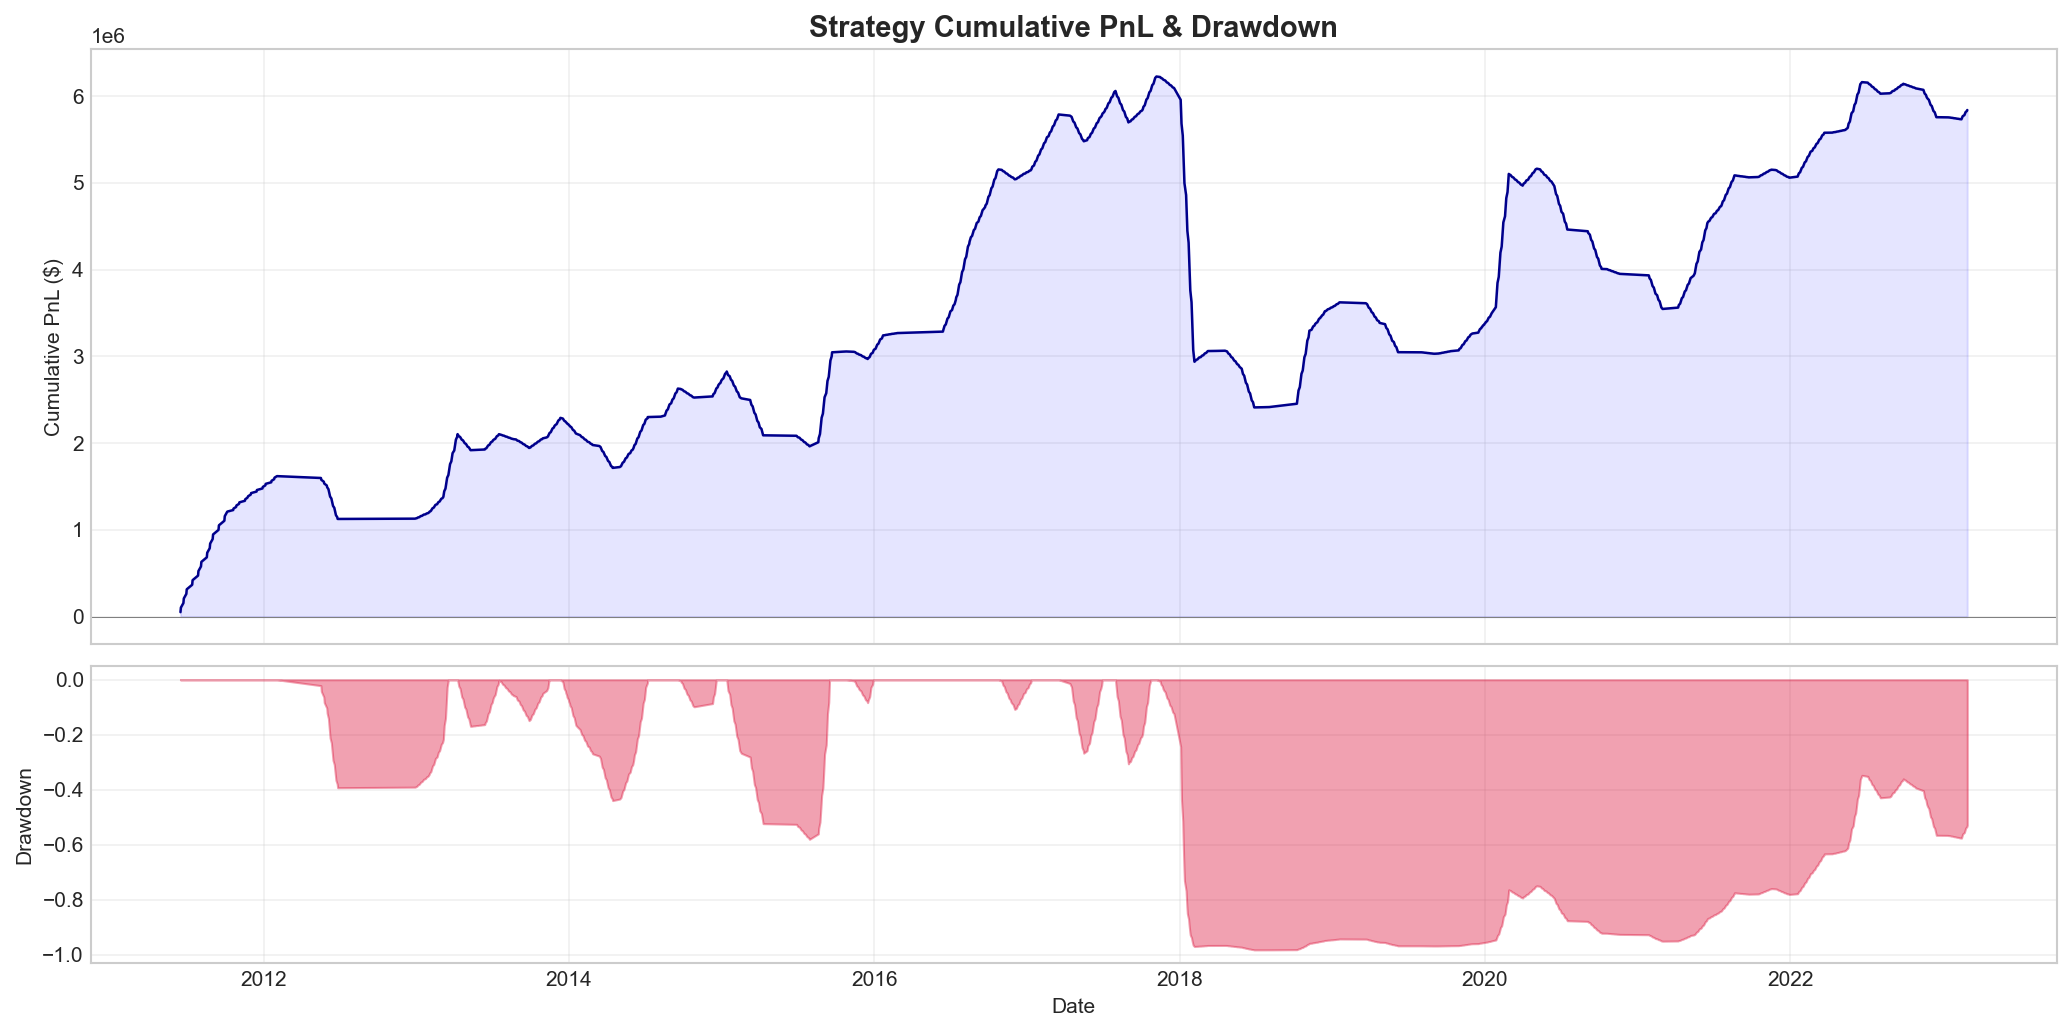
\includegraphics[width=\textwidth]{07_cumulative_pnl.png}
      \end{adjustbox}
      \vspace{-0.3em}
      \scriptsize Cumulative PnL and drawdown (25\% stop per trade, early + expiry).
    \end{column}
    \begin{column}{0.48\textwidth}
      \begin{adjustbox}{max width=\linewidth,max height=0.52\textheight,keepaspectratio}
        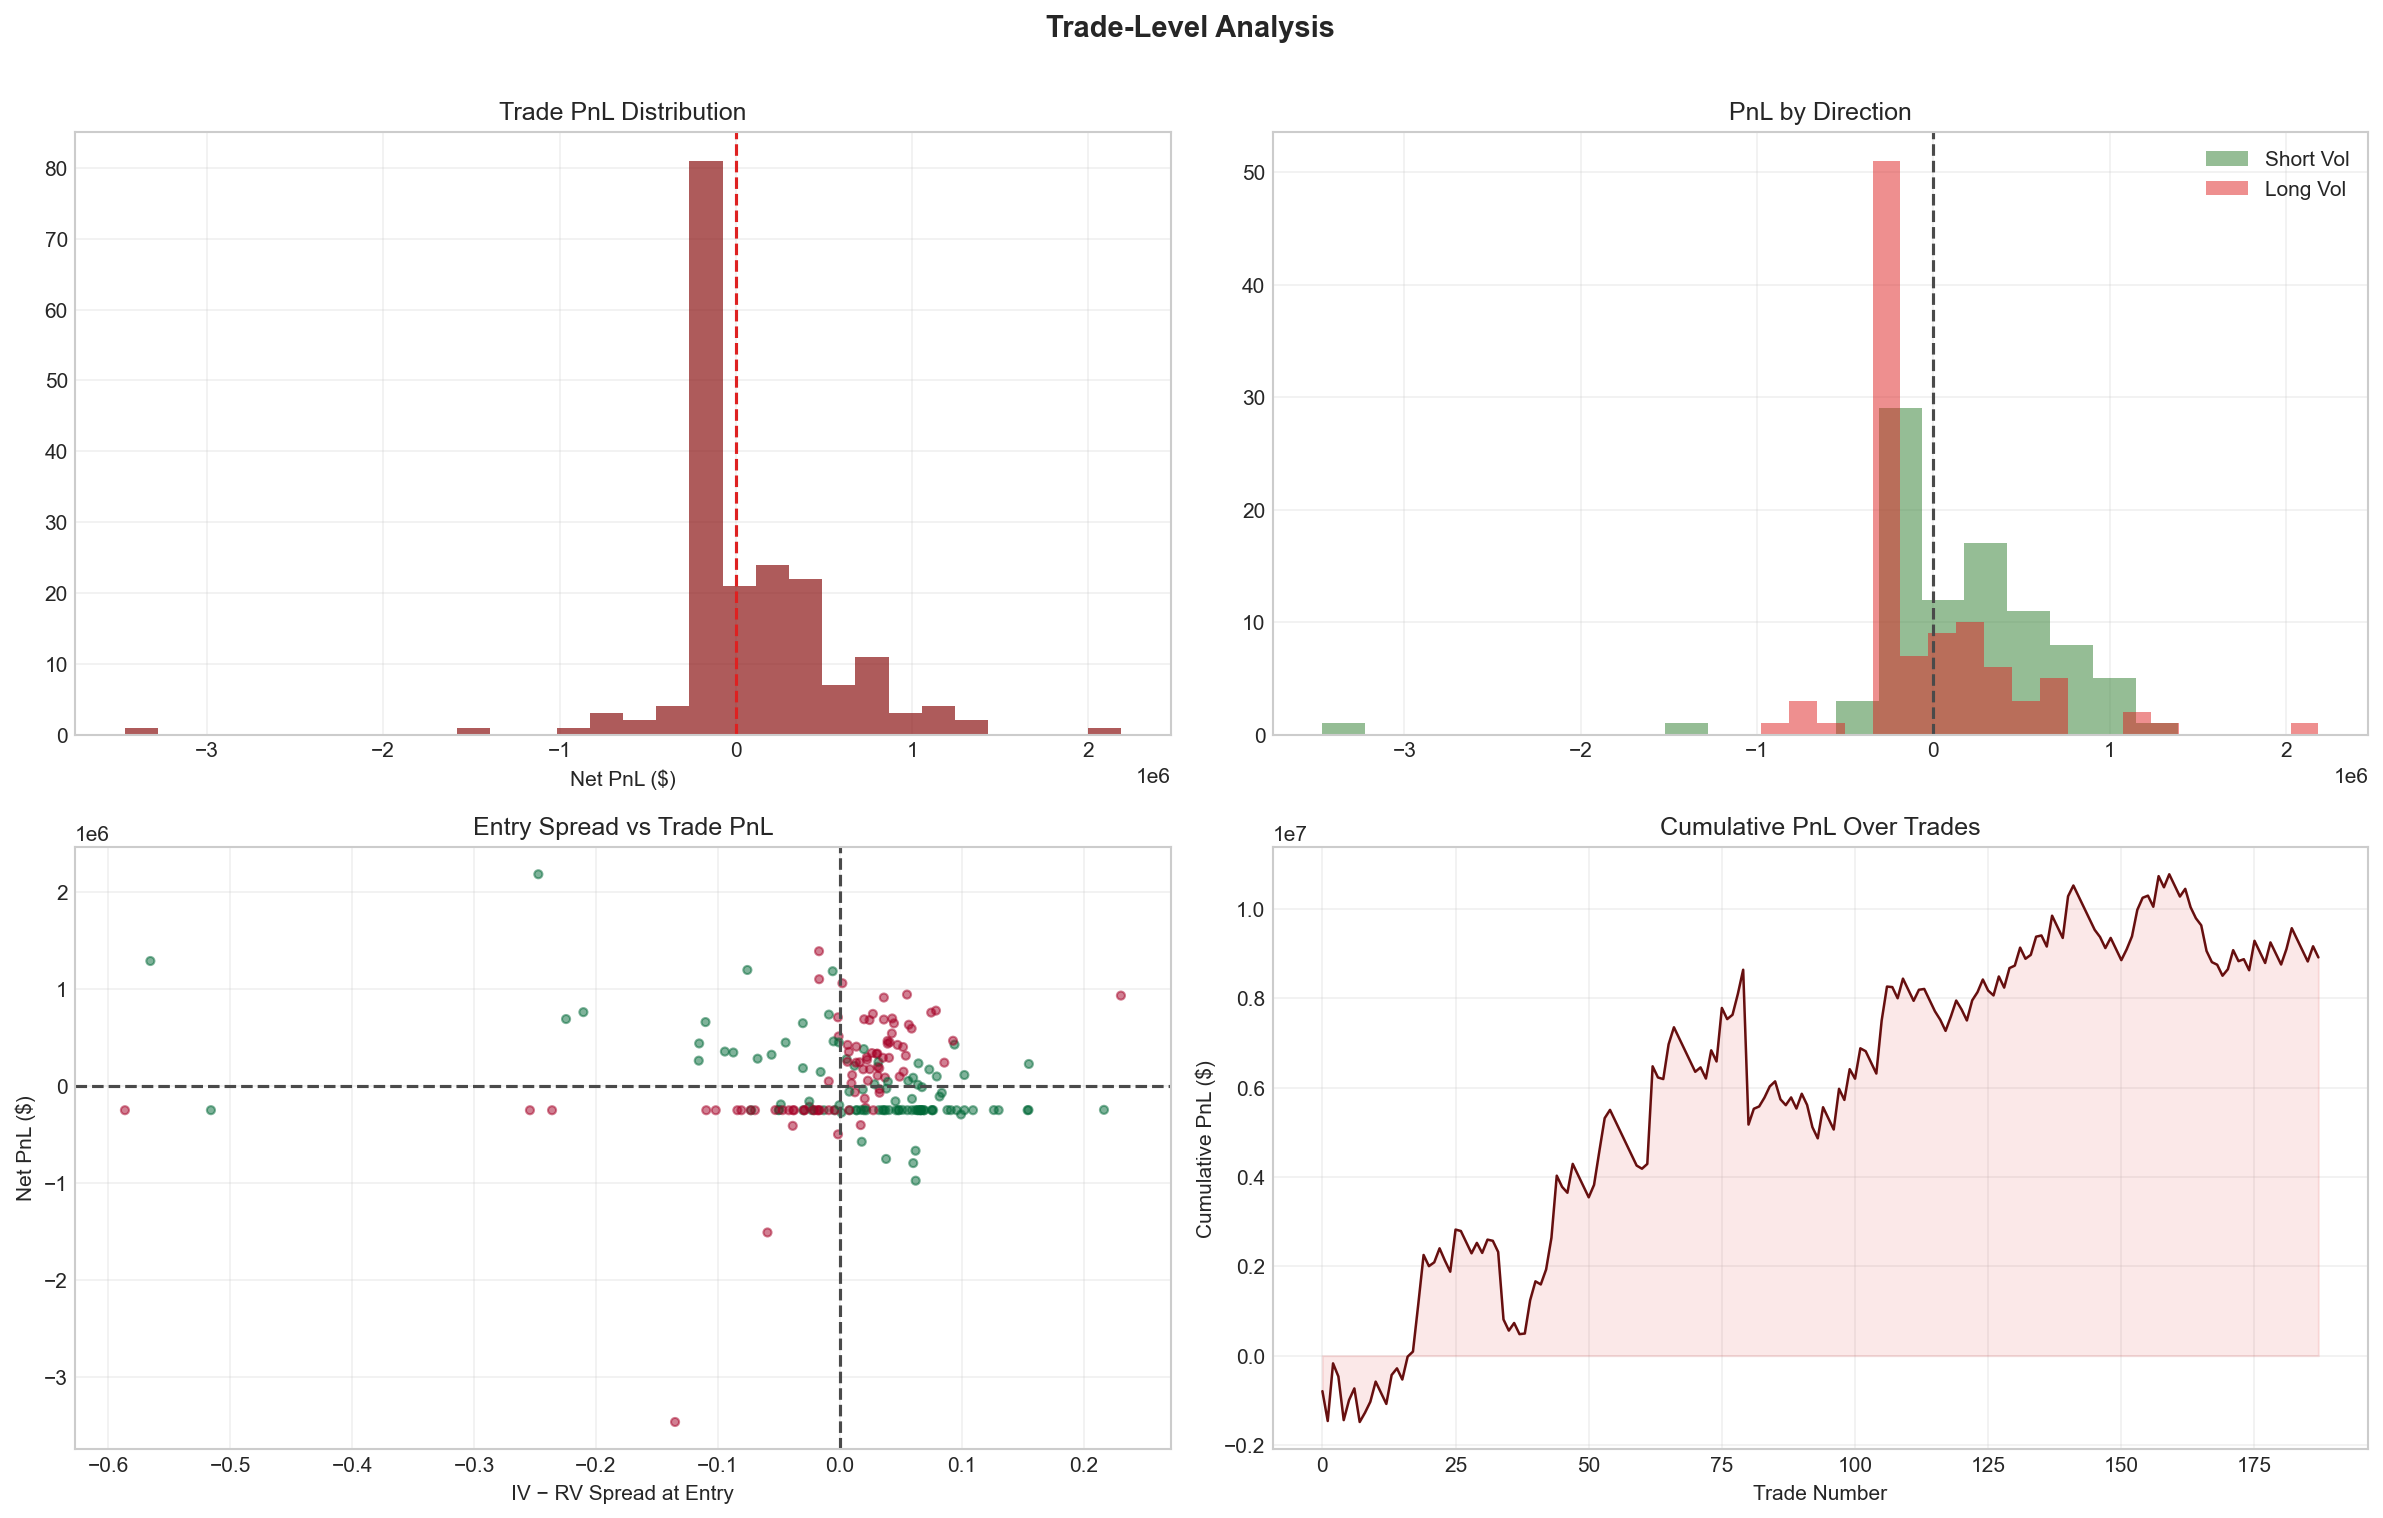
\includegraphics[width=\textwidth]{08_trade_analysis.png}
      \end{adjustbox}
      \vspace{-0.3em}
      \scriptsize PnL distribution, IV vs RV at entry, direction breakdown.
    \end{column}
  \end{columns}
\end{frame}

\begin{frame}{Monthly Returns \& Key Metrics}
  \centering
  \begin{adjustbox}{max width=\textwidth,max height=0.58\textheight,keepaspectratio}
    
\includegraphics[width=\textwidth]{09_monthly_returns.png}
  \end{adjustbox}\\
  \scriptsize \centering Monthly return heatmap. \\
  \footnotesize
  \textbf{Full-sample (VRP, 25\% stop):} 188 trades, 46.3\% win, \$16.54M total PnL; Sharpe 2.16, Sortino 4.43, Calmar 2.91; Ann.\ return 244\%, vol 67.1\%, max DD $-$83.9\%; Benchmark (SPX): Sharpe 0.66; alpha 324\%, info ratio 3.41.
\end{frame}

\begin{frame}{Robustness \& Parameter Sensitivity (Pipeline)}
  \begin{columns}[T]
    \begin{column}{0.48\textwidth}
      \begin{adjustbox}{max width=\linewidth,max height=0.52\textheight,keepaspectratio}
        
\includegraphics[width=\textwidth]{10_robustness_subperiods.png}
      \end{adjustbox}
      \vspace{-0.3em}
      \scriptsize Sharpe by sub-period.
    \end{column}
    \begin{column}{0.48\textwidth}
      \begin{adjustbox}{max width=\linewidth,max height=0.52\textheight,keepaspectratio}
        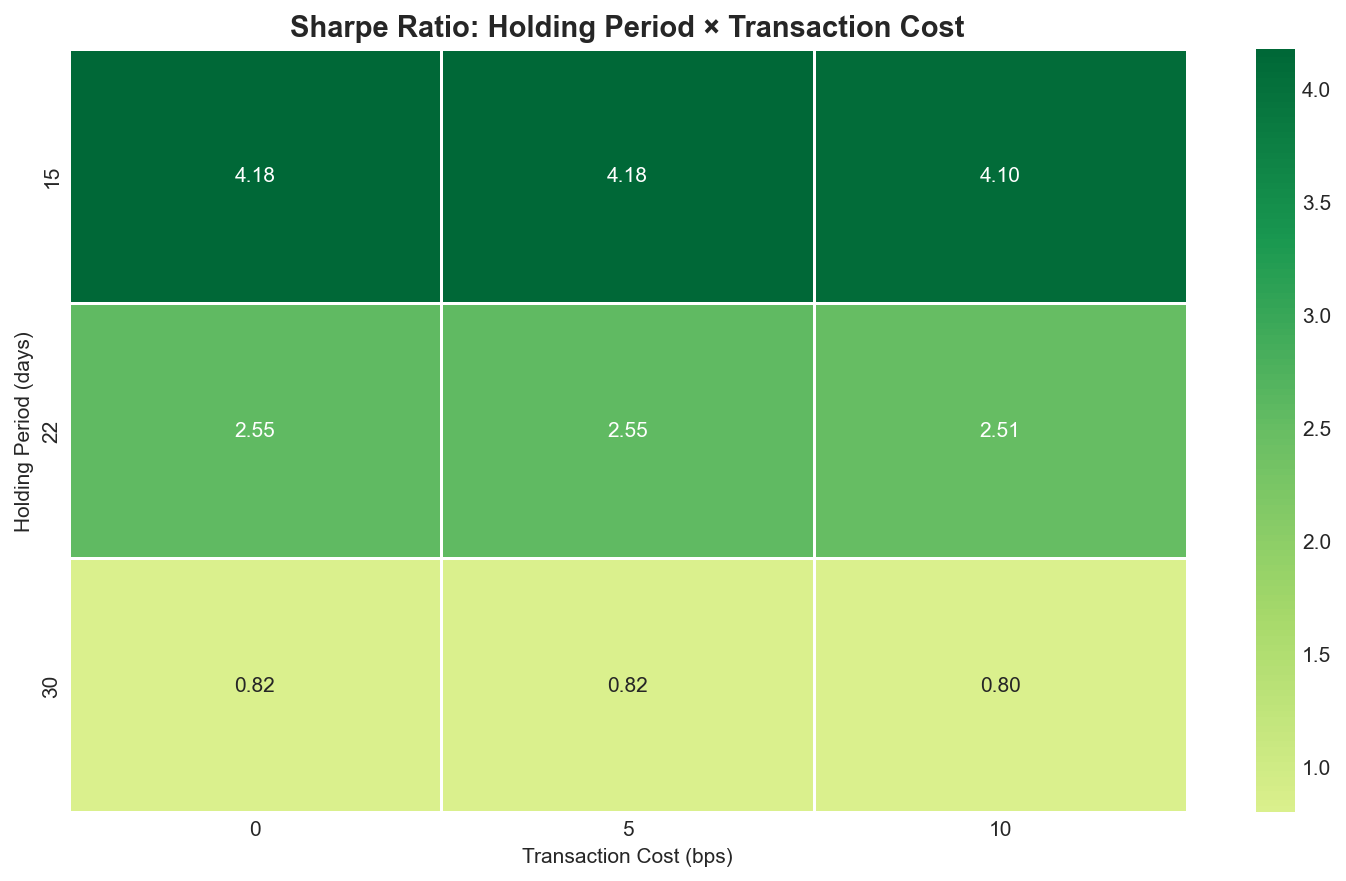
\includegraphics[width=\textwidth]{11_parameter_sensitivity.png}
      \end{adjustbox}
      \vspace{-0.3em}
      \scriptsize Sharpe across hold days $\times$ cost (bps).
    \end{column}
  \end{columns}
\end{frame}

\begin{frame}{Summary Dashboard}
  \centering
  \begin{adjustbox}{max width=\textwidth,max height=0.82\textheight,keepaspectratio}
    
\includegraphics[width=\textwidth]{12_summary_dashboard.png}
  \end{adjustbox}\\
  \scriptsize \centering Six-panel overview: SPX, IV vs RV, VRP signal, cumulative PnL, metrics, drawdown.
\end{frame}

% ═══════════════════════════════════════════════════════════
\section{Strategy Comparison \& FOMC}
% ═══════════════════════════════════════════════════════════

\begin{frame}{Strategy Comparison}
  \centering
  \begin{adjustbox}{max width=\textwidth,max height=0.68\textheight,keepaspectratio}
    
\includegraphics[width=\textwidth]{13_strategy_comparison.png}
  \end{adjustbox}\\
  \scriptsize \centering VRP vs Var Swap: PnL, Sharpe, drawdowns. \\
  \footnotesize
  \textbf{Var Swap leads:} Var Swap: 190 trades, Sharpe 2.54, \$24.89M, max DD $-$82.3\%; VRP: 188 trades, Sharpe 2.16, \$16.54M, max DD $-$83.9\%. 25\% stop per trade caps losses.
\end{frame}

\begin{frame}{Results Comparison: All Strategies}
  \centering
  \scriptsize
  \begin{tabular}{@{}lrrrrr@{}}
    \toprule
    \textbf{Strategy} & \textbf{Trades} & \textbf{Win Rate} & \textbf{Sharpe} & \textbf{Total PnL} & \textbf{Max DD} \\
    \midrule
    VRP (ATM IV, composite RV) & 188 & 46.3\% & 2.16 & \$16.54M & $-$83.9\% \\
    Var Swap (MFIV) & 190 & 48.4\% & 2.54 & \$24.89M & $-$82.3\% \\
    Logistic (RV forecast, $K{=}8$) & 186 & 47.3\% & 2.11 & \$16.62M & $-$84.9\% \\
    \bottomrule
  \end{tabular}
  \vspace{0.5em}
  \normalsize
  \raggedright
  \footnotesize
  Same backtest: delta-hedged straddles, \$1M notional, hold to expiry (1--5d), 25\% stop per trade (early + expiry), 5\,bps cost.
\end{frame}

\begin{frame}{FOMC Window Analysis}
  \centering
  \begin{adjustbox}{max width=\textwidth,max height=0.68\textheight,keepaspectratio}
    
\includegraphics[width=\textwidth]{14_fomc_analysis.png}
  \end{adjustbox}\\
  \scriptsize \centering FOMC $\pm$7d vs non-FOMC across strategies. \\
  \footnotesize
  \textbf{FOMC vs non-FOMC (VRP):} FOMC: 79 trades, 48\% win, \$15.37M, Sharpe 1.65; Non-FOMC: 142 trades, 40\% win, \$17.35M, Sharpe 1.48. Both profitable.
\end{frame}

% ═══════════════════════════════════════════════════════════
\section{OOS, Stress \& Regime}
% ═══════════════════════════════════════════════════════════

\begin{frame}{Out-of-Sample \& Walk-Forward}
  \centering
  \begin{adjustbox}{max width=\textwidth,max height=0.68\textheight,keepaspectratio}
    
\includegraphics[width=\textwidth]{15_oos_walkforward.png}
  \end{adjustbox}\\
  \scriptsize \centering OOS cumulative PnL; walk-forward Sharpe by window. \\
  \footnotesize
  \textbf{OOS (60/40 split):} In-sample: 115 trades, Sharpe 2.86, \$15.10M; Out-of-sample: 73 trades, Sharpe 0.69, \$1.44M. \textbf{Walk-forward:} 5 of 5 windows profitable.
\end{frame}

\begin{frame}{Stress Periods}
  \centering
  \begin{adjustbox}{max width=\textwidth,max height=0.68\textheight,keepaspectratio}
    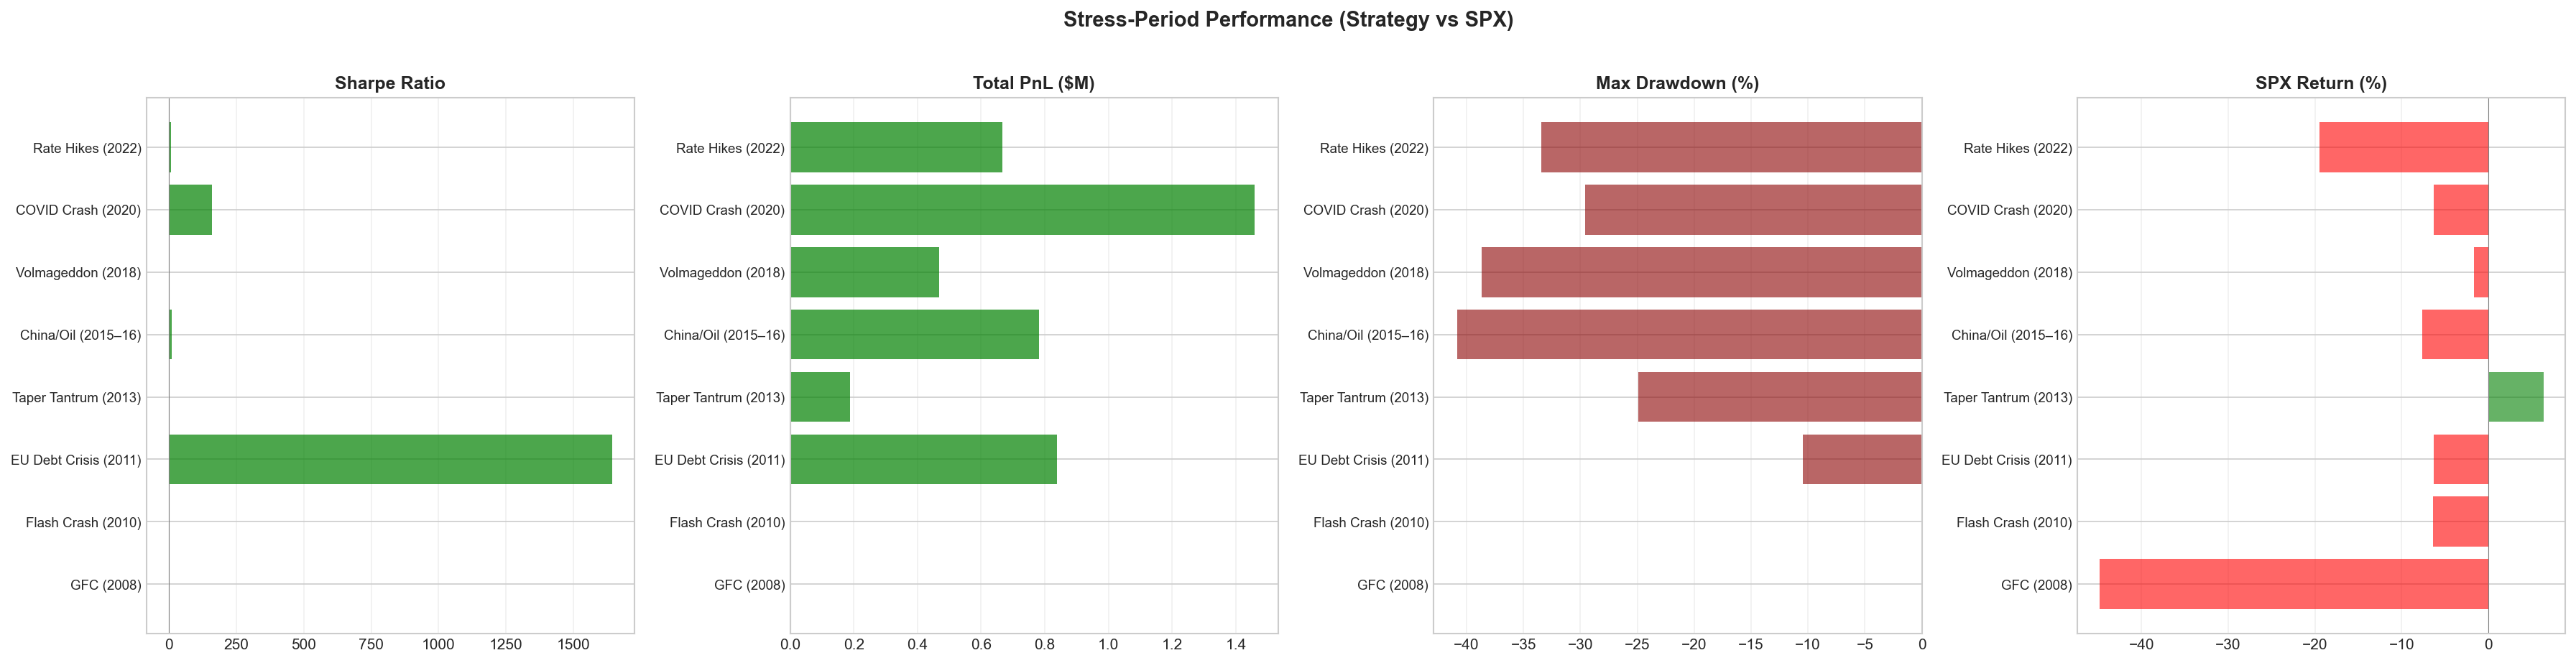
\includegraphics[width=\textwidth]{16_stress_periods.png}
  \end{adjustbox}\\
  \scriptsize \centering Sharpe, PnL, max DD by stress episode. \\
  \footnotesize
  \textbf{Selected episodes:} Volmageddon, China/Oil, COVID: strong (Sharpe 6.96, 3.27, 4.70); 2022 rate hikes: negative (Sharpe $-$1.07).
\end{frame}

\begin{frame}{Volatility Regime}
  \centering
  \begin{adjustbox}{max width=\textwidth,max height=0.68\textheight,keepaspectratio}
    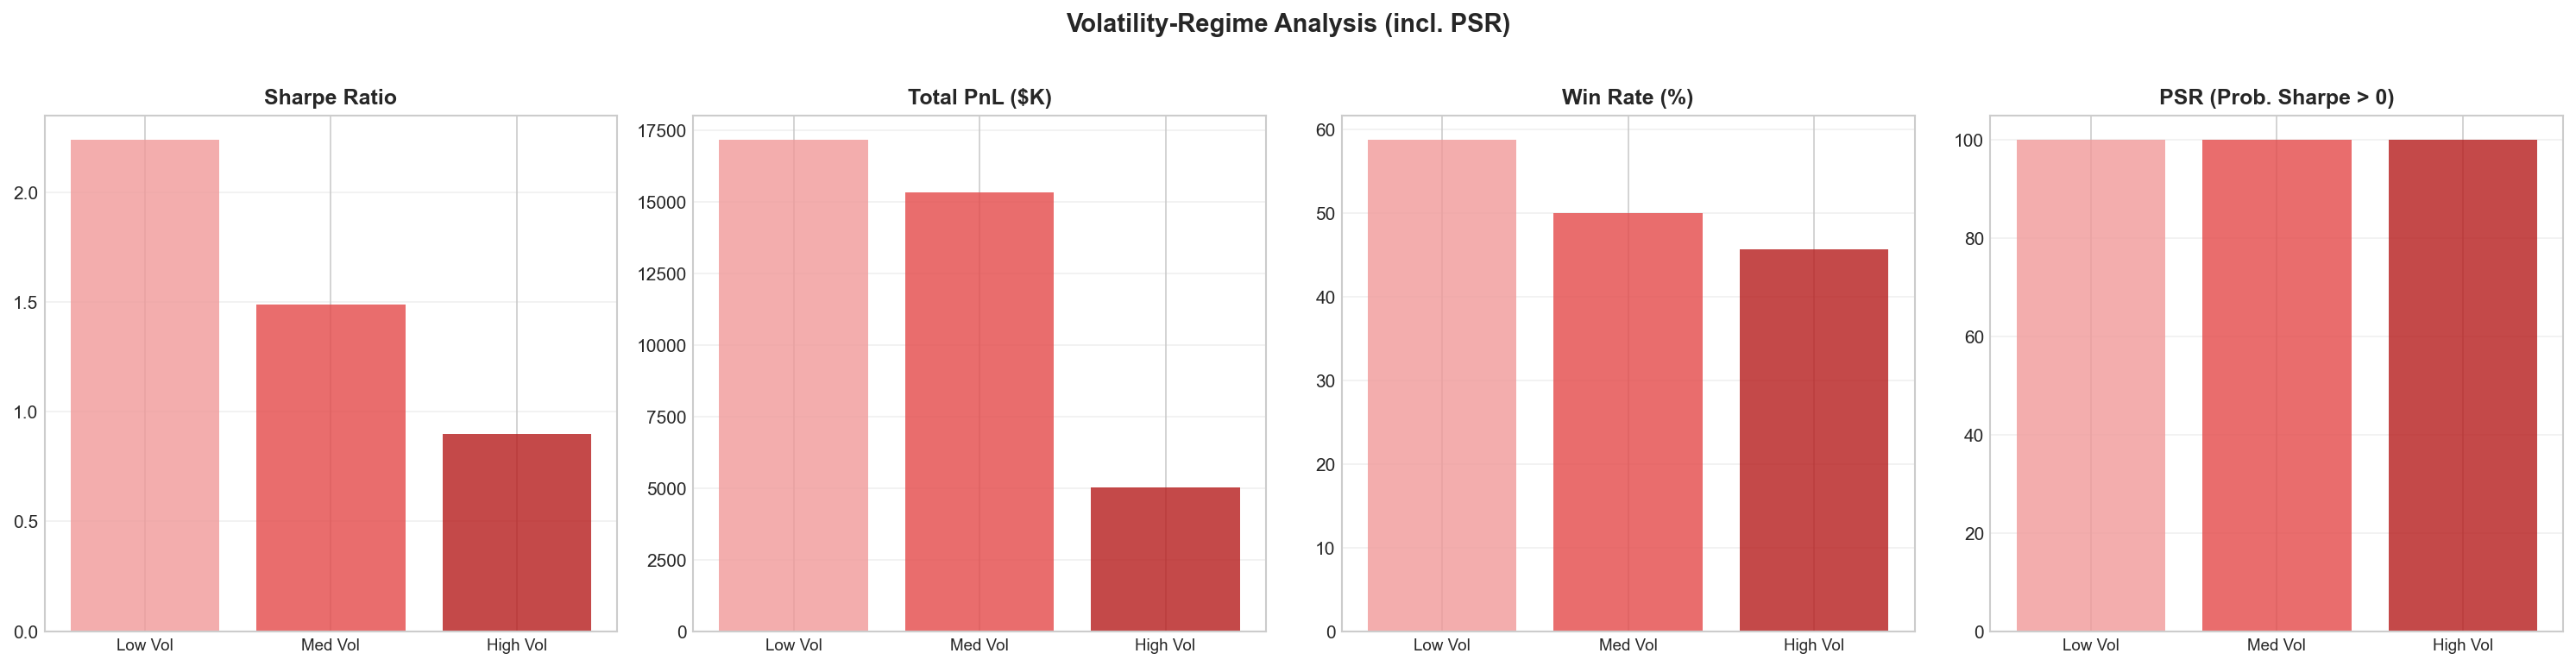
\includegraphics[width=\textwidth]{17_regime_analysis.png}
  \end{adjustbox}\\
  \scriptsize \centering Performance by trailing 252d RV tercile. \\
  \footnotesize
  \textbf{Regime (VRP):} Low vol: \$17.17M, Sharpe 2.24; Medium vol: \$15.32M, Sharpe 1.49; High vol: \$5.02M, Sharpe 0.90. Profitable across regimes; best in low vol.
\end{frame}

% ═══════════════════════════════════════════════════════════
\section{Parameter Sensitivity \& Inference}
% ═══════════════════════════════════════════════════════════

\begin{frame}{Parameter Sensitivity (Robustness)}
  \centering
  \begin{adjustbox}{max width=\textwidth,max height=0.68\textheight,keepaspectratio}
    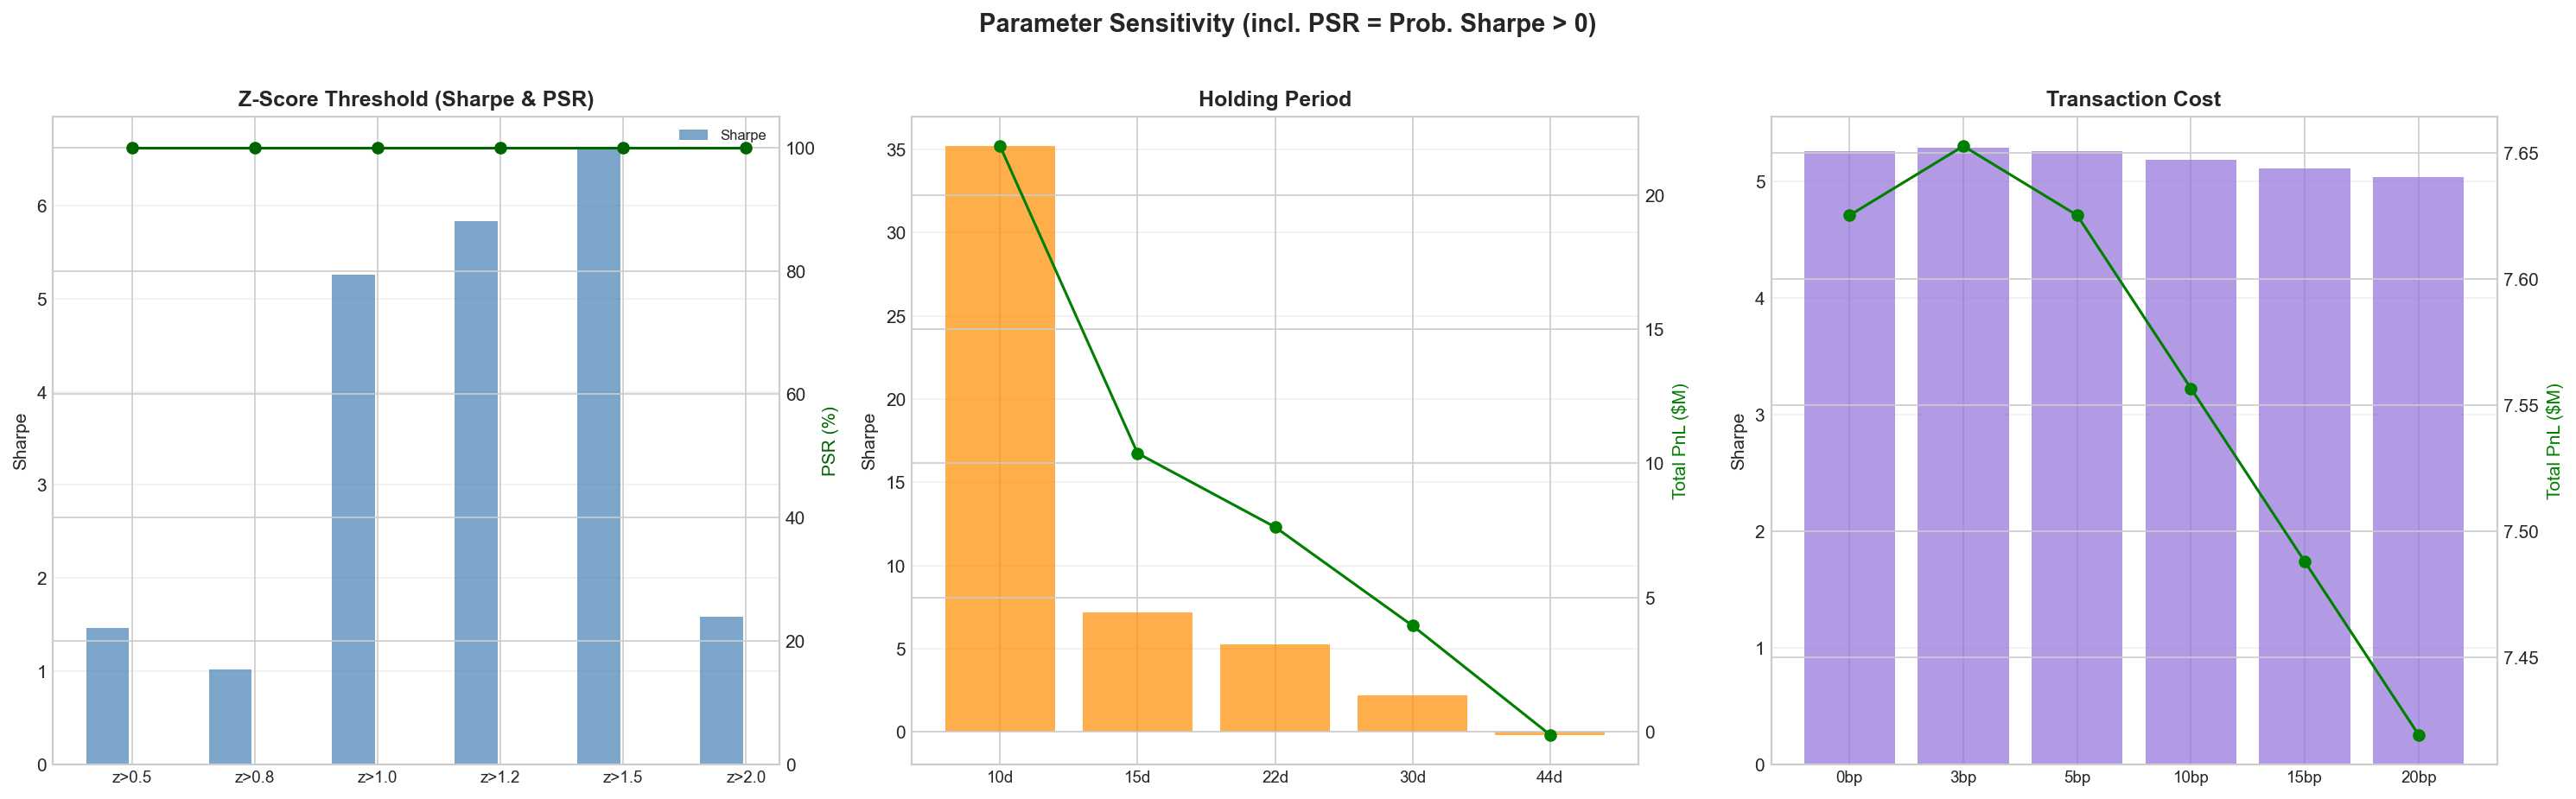
\includegraphics[width=\textwidth]{18_param_sensitivity.png}
  \end{adjustbox}\\
  \scriptsize \centering Z-threshold, hold days, transaction cost. \\
  \footnotesize
  \textbf{Findings:} Z-threshold: Sharpe positive across grid; degrades at $z > 1.5$. Hold: stable at 2.16 for 1--5d (weeklies). Cost: robust 0--20\,bps.
\end{frame}

\begin{frame}{Bootstrap Sharpe \& Yearly Breakdown}
  \begin{columns}[T]
    \begin{column}{0.48\textwidth}
      \begin{adjustbox}{max width=\linewidth,max height=0.52\textheight,keepaspectratio}
        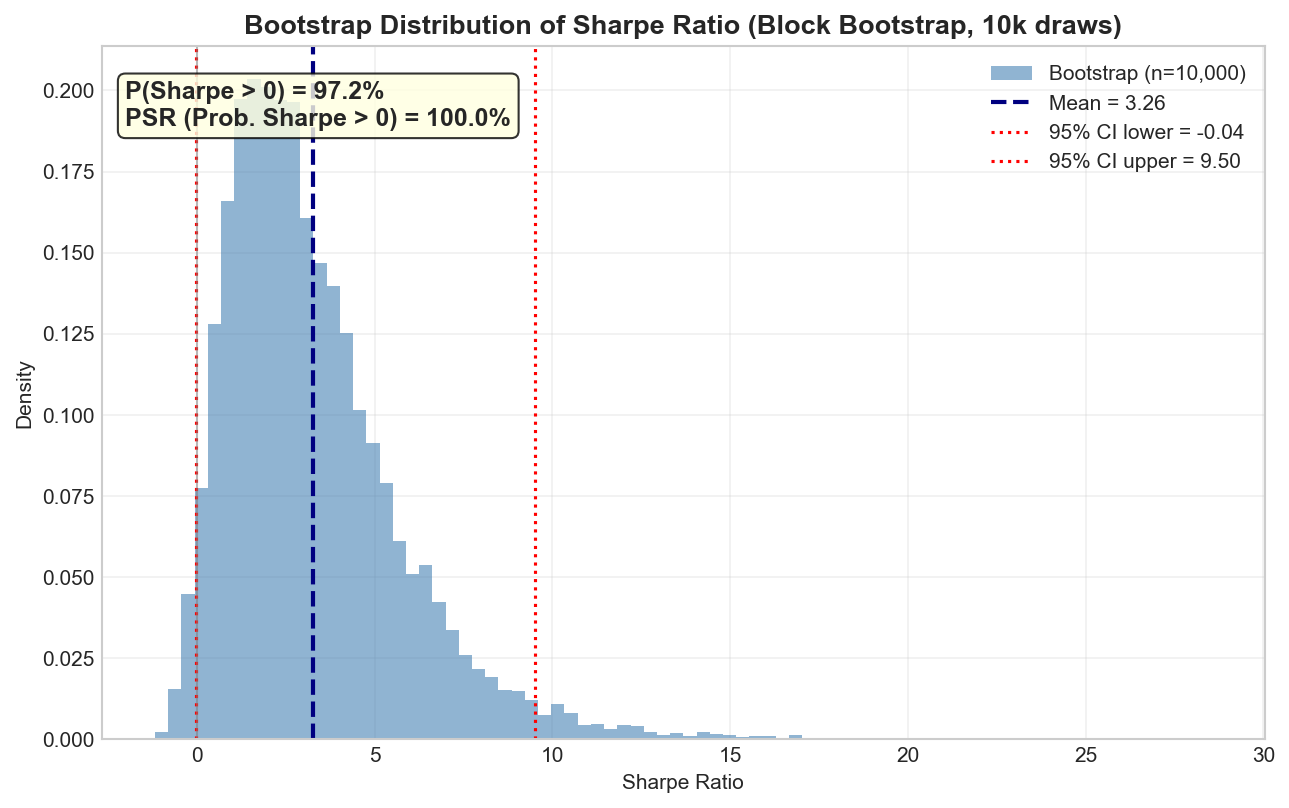
\includegraphics[width=\textwidth]{19_bootstrap_sharpe.png}
      \end{adjustbox}
      \vspace{-0.3em}
      \scriptsize Block bootstrap (10k, 22-day blocks); 95\% CI, P(Sharpe $>$ 0).
    \end{column}
    \begin{column}{0.48\textwidth}
      \begin{adjustbox}{max width=\linewidth,max height=0.52\textheight,keepaspectratio}
        
\includegraphics[width=\textwidth]{20_yearly_breakdown.png}
      \end{adjustbox}
      \vspace{-0.3em}
      \scriptsize Annual Sharpe, PnL, win rate, max DD (2011--2023). Profitable 11 of 13 years; \$16.54M cumulative.
    \end{column}
  \end{columns}
\end{frame}

% ═══════════════════════════════════════════════════════════
\section{Conclusion}
% ═══════════════════════════════════════════════════════════

\begin{frame}{Summary}
  \begin{itemize}
    \item VRP (IV $-$ forecast RV) is \textbf{tradeable} on SPX with delta-hedged straddles.
    \item Sharpe 2.16, \$16.54M PnL (188 trades); Var Swap: Sharpe 2.54, \$24.89M (190 trades). Max DD $\approx$ 84\% (25\% stop per trade caps losses).
    \item Var Swap outperforms VRP on Sharpe and PnL; strong in stress (Volmageddon, COVID); regime-dependent (low-vol best).
    \item \textbf{Logistic regression:} alternative RV forecast (quantiles $\to$ $E[z^2]$ $\to$ expected vol); Sharpe 2.11, \$16.62M at $K{=}8$; composite RV slightly better.
    \item Robust to threshold and costs; hold to expiry (1--5d for weeklies).
  \end{itemize}
\end{frame}

\begin{frame}{Limitations \& Downfalls}
  \begin{itemize}
    \item \textbf{Tail risk:} $\approx$84\% max DD; 25\% stop per trade (early + expiry) caps each loss; assumes executable at cap.
    \item \textbf{Regime-dependent:} Best in low vol (Sharpe 2.24); weaker in high vol (Sharpe 0.90).
    \item \textbf{FOMC:} Both FOMC and non-FOMC windows profitable (Sharpe 1.65 vs 1.48).
    \item \textbf{Statistical uncertainty:} Bootstrap P(Sharpe $>$ 0) = 99.9\%; 95\% CI [0.86, 10.31].
    \item \textbf{Single underlying:} SPX only; one position at a time; limited capacity.
    \item \textbf{Simplified hedging:} Daily delta hedge; no intraday gamma; costs may be optimistic in stress.
  \end{itemize}
\end{frame}

\begin{frame}[c]
  \centering \Large Thank you \\
  \vspace{1em}
  \normalsize Questions?
\end{frame}

\end{document}
